\chapter{Propuesta del proyecto}
\label{chapter:proposed-method}

Este capitulo describe los componentes que integran el metodo propuesto, asi
como la maera en como estos componentes proveen de apoyo al sistema final, este
capitulo esta dividido en dos secciones la primera siendo la seccion
\ref{section:used-method} en donde se explican los conceptos propuestos y
utilizados en el proyecto, esta seccion se divide en varias subsecciones en
donde se explican partes de la propuesta y el como permitiran que el sistema
generado cumpla con los objetivos requeridos, la segunda parte siendo la seccion
\ref{section:previous-proposed-methods} explica ideas y conceptos que se
propusieron a lo largo del desarrollo, el como estos ayudarian a mejorar el
sistema generado.

\section{Propuesta utilizada}
\label{section:used-method}

La propuesta final utilizada en el proyecto esta basada en el uso de varias
tecnicas para la generacion de los compuestos y subsecuentemente los niveles
para el juego de Angry Birds, la base de todo el proyecto esta en el uso de un
algoritmo genetico para evolucionar los individuos, esto se explica mas a
detalle en la seccion \ref{subsection:generate-levels-using-GA}

\subsection{Generar compuestos de piezas base}
\label{subsection:generate-composites}

El videojuego de Angry Birds cuenta con un total de 11 diferentes tipos de
bloques, ademas de 2 grupos de objetos siendo estos cajas de explosivos y los
puercos que pueden ser colocados en el nivel, ademas de esto cuenta con
plataformas que pueden ser agregadas y rotadas para establecer plataformas en
donde colocar mas bloques, de estos solo utilizaremos las 11 piezas basicas
mostradas en la figura \ref{figure:game-basic-blocks} y los puercos para generar
niveles.

Las piezas basicas no pueden ser modificadas, tampoco es posible agregar nuevos
bloques al codigo debido a que la competencia solo utiliza las piezas regulares,
para poder librar esta restriccion se generaran compuestos con las piezas base,
estos compuestos pueden estar formados de 1, 2 o mas bloques basicos, estos
grupos se utilizaran para generar las estructuras que se colocaran en los niveles.

\begin{figure}
  \centering
  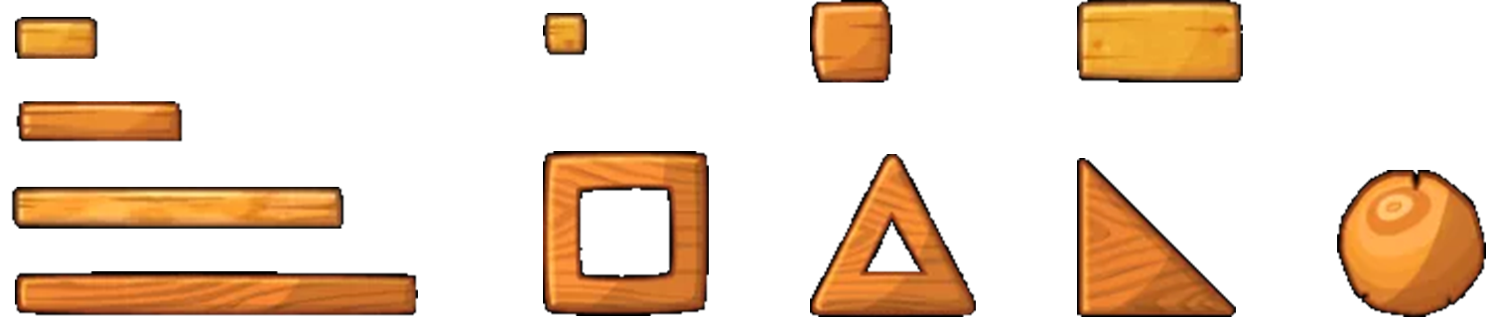
\includegraphics[width=1.0\textwidth]{img/list_pieces.png}
  \caption{Piezas basicas del juego angry birds}
  \label{figure:game-basic-blocks}
\end{figure}

La manera porpuesta para generar estos conjuntos es mediante el uso de los
valores de alto y ancho de las piezas para poder definir los bordes de las
mismas, de esta manera al momento de querer unir dos o mas piezas para formar un
conjunto la medida del conjunto se calculara buscando el punto mas alto, mas
bajo asi como las posiciones mas a la derecha e izquierda teniendo ambas piezas
unidas, un ejemplo de la union de cuatro piezas se muestra en la figura
\ref{figure:bounding-box-calculation} en donde cuatro piezas se colocan unas
sobre otras para formar un objeto cuadrado, para poder agregar las piezas como
un conjunto se buscan los puntos mas alejados, una vez que se ah calculado el
alto y ancho del conjunto se procede a encontrar el punto central del mismo,
desde este punto se calcula la distancia en \textit{x} y \textit{y} hacia los
centros de cada una de las piezas del conjnto, estos valores de centros se
agregan en manera de diccionario para poder genererar los objetos requeridos al
momento de crear a los individuos antes de iniciar las generaciones.

\begin{figure}
  \centering
  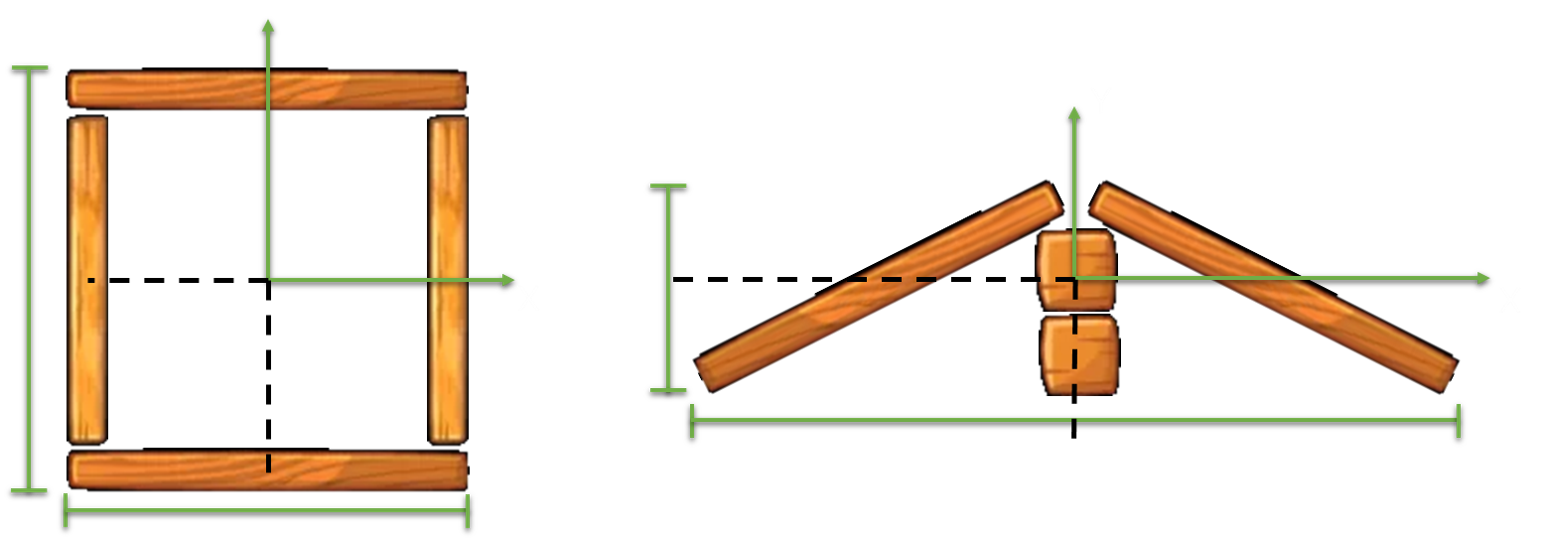
\includegraphics[width=1.0\textwidth]{img/bounding_box_calculation.png}
  \caption{Calculo de bordes de un conjunto}
  \label{figure:bounding-box-calculation}
\end{figure}

Debido a que los conjuntos son creados antes de la ejecucion del algoritmo se
permite que el algoritmo se base unicamente manteniendo los apuntadores a las
composiciones de piezas y solo trabaja con estas mendiante las operaciones
geneticas del propio algoritmo, esto permitira que el algoritmo utilize menos
tiempo identificando posibles composiciones.

Utilizando esta manera de generar los compuestos simplemente se utiliza un
algoritmo basado en clases para poder acomodar los elementos y crear los objetos
requeridos segun sean necesarios, esto se explica mas detalladamente en la
seccion \ref{subsection:classorientedidea}.

\subsection{Generacion de compuestos mediante objetos de clase}
\label{subsection:classorientedidea}

Para mantener un control de los compuestos, principalmente de las piezas
individuales que forman los compuestos se propuso la generacion de clases con
herencia en donde una clase principal contendra los metodos que las clases hijas
utilizaran para obtener valores especificos cuando las piezas requieran,
principalmente estos metodos se encargan de calcular las esquinas de las piezas
particulares las cuales permitiran una vez se tenga un conjunto encontrar la
altura y tamaño total del conjunto asi como el centro del mismo.

Utilizando la estrategia mostrada en la figura
\ref{figure:bounding-box-calculation} y explicada en el capitulo anterior se
define una clase para los conjuntos de piezas, aqui se utilizan los calculos de
las clases particulares anteriorente mencionadas para obtener los valores de
bordes y tamaño de los conjuntos, estas clases se crean deacuerdo a los
apuntadores indicados en los individuaos de la poblacion, cuando un apuntador
hace referencia a un grupo se obtienen los datos de la piezas que integran al
conjunto y se crean objetos nuevos de esas mismas clases que perteneceran a un
individuo particular, esto debido a que al hacer referencia a un objeto
previamente creado un cambio realizado en un individuo particular se propagaria
a todos los individuos que utilizen ese mismo apuntador, por tal motivo cuando
se crean los conjuntos se mantiene una lista de valores que indican la clase que
se debera de crear y la posicion en \textit{x} y \textit{y} relativa al centro
del mismo conjunto.

El sistema de clases se establecio con el fin de reducir la redundancia de
codigo y para permitir que cada clase particular mantenga los datos necesarios
para crear los objetos que contiene asi como mantener las listas de las piezas
que conforman los niveles antes y despues de haber realizado las simulaciones
para poder realizar los calculos de manera mas rapida ademas de las clases que
controlan los conjuntos y subsecuentemente las piezas individuales. 

\begin{figure}
  \centering
  %%%%%%%%%%%%%%%%%%%%%%%%%%%%%%%%%%%%%%%%%%%%%%%%%%%%%%%%%%%%%%%%
% Class diagram
% Author: Salinas Hernández Jaime
% Version: 1.0 
%%%%%%%%%%%%%%%%%%%%%%%%%%%%%%%%%%%%%%%%%%%%%%%%%%%%%%%%%%%%%%%
\tikzstyle{abstract}=[rectangle, draw=black, rounded corners, fill=blue!40, drop shadow,
        text centered, anchor=north, text=white, text width=4.2cm]
\tikzstyle{comment}=[rectangle, draw=black, rounded corners, fill=green, drop shadow,
        text centered, anchor=north, text=white, text width=4.2cm]
\tikzstyle{myarrow}=[->, >=open triangle 90, thick]
\tikzstyle{line}=[-, thick]
        

\begin{tikzpicture}[node distance=2cm]
    \node (Item) [abstract, rectangle split, align=left, rectangle split parts=3]
        {
            \textbf{Pieza}
            \nodepart{second}string: Material \newline float: X \newline float: Y \newline float: Z \newline
            \nodepart{third}get\_edges \newline as\_dictionary \newline get\_points \newline update\_values
        };
    %\node (ItemInstants) [comment, rectangle split, rectangle split parts=2, below=0.2cm of Item, text justified]
    %    {
    %        \textbf{Methods}
    %        \nodepart{second}
    %            get\_edges
    %            \newline as\_dictionary
    %            \newline get\_points
    %            \newline update\_values
    %    };
    \node (AuxNode01) [text width=4cm, below=3cm of Item] {};
    
    \node (Circle) [abstract, rectangle split, align=left, rectangle split parts=2, left=of AuxNode01]
        {
            \textbf{Circle}
            \nodepart{second}text: "Circle" \newline
            int: Height = 75 \newline
            int: Width = 75
        };
    \node (RectTiny) [abstract, rectangle split, align=left, rectangle split parts=2, right=of Circle]
        {
            \textbf{RectTiny}
            \nodepart{second}text: "RectTiny"\newline int: Height = 25 \newline int: Width = 45
        };
    \node (RectSmall) [abstract, rectangle split, align=left, rectangle split parts=2, right=of RectTiny]
        {
            \textbf{RectSmall}
            \nodepart{second}text: "RectSmall"\newline int: Height = 25 \newline int: Width = 85
        };
    \node (RectMedium) [abstract, rectangle split, align=left, rectangle split parts=2, right=of RectSmall]
        {
            \textbf{RectMedium}
            \nodepart{second}text: "RectMedium"\newline int: Height = 25 \newline int: Width = 165
        };
    \node (RectBig) [abstract, rectangle split, align=left, rectangle split parts=2, right=of RectMedium]
        {
            \textbf{RectBig}
            \nodepart{second}text: "RectBig"\newline int: Height = 25 \newline int: Width = 185
        };
    
    
        
    \node (AuxNode02) [text width=0.5cm, below=of Circle] {};   
    
    \node (RectFat) [abstract, rectangle split, align=left, rectangle split parts=2, left=of AuxNode02]
        {
            \textbf{RectFat}
            \nodepart{second}text: "RectFat"\newline int: Height = 25 \newline int: Width = 85
        };
    \node (SquareTiny) [abstract, rectangle split, align=left, rectangle split parts=2, right=of RectFat]
        {
            \textbf{SquareTiny}
            \nodepart{second}text: "SquareTiny"\newline int: Height = 25 \newline int: Width = 25
        };
    \node (SquareSmall) [abstract, rectangle split, align=left, rectangle split parts=2, right=of SquareTiny]
        {
            \textbf{SquareSmall}
            \nodepart{second}text: "SquareSmall"\newline int: Height = 45 \newline int: Width = 45
        };
    \node (Triangle) [abstract, rectangle split, align=left, rectangle split parts=2, right=of SquareSmall]
        {
            \textbf{Triangle}
            \nodepart{second}text: "Triangle"\newline int: Height = 75 \newline int: Width = 75
        };
    \node (TriangleHole) [abstract, rectangle split, align=left, rectangle split parts=2, right=of Triangle]
        {
            \textbf{TriangleHole}
            \nodepart{second}text: "TriangleHole"\newline int: Height = 85 \newline int: Width = 85
        };
    \node (SquareHole) [abstract, rectangle split, align=left, rectangle split parts=2, right=of TriangleHole]
        {
            \textbf{SquareHole}
            \nodepart{second}text: "SquareHole"\newline int: Height = 85 \newline int: Width = 85
        };
        
    
    
    \draw[myarrow] (RectSmall.north) -- ++(0,0.8) -| (Item.south);
    \draw[line] (Circle.north) -- ++(0,0.8) -| (RectTiny.north);
    \draw[line] (Circle.north) -- ++(0,0.8) -| (RectSmall.north);
    \draw[line] (Circle.north) -- ++(0,0.8) -| (RectMedium.north);
    \draw[line] (Circle.north) -- ++(0,0.8) -| (RectBig.north);
    \draw[line] (Circle.north) -- ++(0,0.8) -| (RectFat.north);
    \draw[line] (Circle.north) -- ++(0,0.8) -| (SquareTiny.east);
    \draw[line] (Circle.north) -- ++(0,0.8) -| (SquareSmall.east);
    \draw[line] (Circle.north) -- ++(0,0.8) -| (Triangle.east);
    \draw[line] (Circle.north) -- ++(0,0.8) -| (TriangleHole.east);
    \draw[line] (Circle.north) -- ++(0,0.8) -| (SquareHole.east);
        
        
\end{tikzpicture}
  \scalebox{.43}{%%%%%%%%%%%%%%%%%%%%%%%%%%%%%%%%%%%%%%%%%%%%%%%%%%%%%%%%%%%%%%%
% Class diagram
% Author: Salinas Hernández Jaime
% Version: 1.0 
%%%%%%%%%%%%%%%%%%%%%%%%%%%%%%%%%%%%%%%%%%%%%%%%%%%%%%%%%%%%%%%
\tikzstyle{abstract}=[rectangle, draw=black, rounded corners, fill=blue!40, drop shadow,
        text centered, anchor=north, text=white, text width=4.2cm]
\tikzstyle{comment}=[rectangle, draw=black, rounded corners, fill=green, drop shadow,
        text centered, anchor=north, text=white, text width=4.2cm]
\tikzstyle{myarrow}=[->, >=open triangle 90, thick]
\tikzstyle{line}=[-, thick]
        

\begin{tikzpicture}[node distance=2cm]
    \node (Item) [abstract, rectangle split, align=left, rectangle split parts=3]
        {
            \textbf{Pieza}
            \nodepart{second}string: Material \newline float: X \newline float: Y \newline float: Z \newline
            \nodepart{third}get\_edges \newline as\_dictionary \newline get\_points \newline update\_values
        };
    %\node (ItemInstants) [comment, rectangle split, rectangle split parts=2, below=0.2cm of Item, text justified]
    %    {
    %        \textbf{Methods}
    %        \nodepart{second}
    %            get\_edges
    %            \newline as\_dictionary
    %            \newline get\_points
    %            \newline update\_values
    %    };
    \node (AuxNode01) [text width=4cm, below=3cm of Item] {};
    
    \node (Circle) [abstract, rectangle split, align=left, rectangle split parts=2, left=of AuxNode01]
        {
            \textbf{Circle}
            \nodepart{second}text: "Circle" \newline
            int: Height = 75 \newline
            int: Width = 75
        };
    \node (RectTiny) [abstract, rectangle split, align=left, rectangle split parts=2, right=of Circle]
        {
            \textbf{RectTiny}
            \nodepart{second}text: "RectTiny"\newline int: Height = 25 \newline int: Width = 45
        };
    \node (RectSmall) [abstract, rectangle split, align=left, rectangle split parts=2, right=of RectTiny]
        {
            \textbf{RectSmall}
            \nodepart{second}text: "RectSmall"\newline int: Height = 25 \newline int: Width = 85
        };
    \node (RectMedium) [abstract, rectangle split, align=left, rectangle split parts=2, right=of RectSmall]
        {
            \textbf{RectMedium}
            \nodepart{second}text: "RectMedium"\newline int: Height = 25 \newline int: Width = 165
        };
    \node (RectBig) [abstract, rectangle split, align=left, rectangle split parts=2, right=of RectMedium]
        {
            \textbf{RectBig}
            \nodepart{second}text: "RectBig"\newline int: Height = 25 \newline int: Width = 185
        };
    
    
        
    \node (AuxNode02) [text width=0.5cm, below=of Circle] {};   
    
    \node (RectFat) [abstract, rectangle split, align=left, rectangle split parts=2, left=of AuxNode02]
        {
            \textbf{RectFat}
            \nodepart{second}text: "RectFat"\newline int: Height = 25 \newline int: Width = 85
        };
    \node (SquareTiny) [abstract, rectangle split, align=left, rectangle split parts=2, right=of RectFat]
        {
            \textbf{SquareTiny}
            \nodepart{second}text: "SquareTiny"\newline int: Height = 25 \newline int: Width = 25
        };
    \node (SquareSmall) [abstract, rectangle split, align=left, rectangle split parts=2, right=of SquareTiny]
        {
            \textbf{SquareSmall}
            \nodepart{second}text: "SquareSmall"\newline int: Height = 45 \newline int: Width = 45
        };
    \node (Triangle) [abstract, rectangle split, align=left, rectangle split parts=2, right=of SquareSmall]
        {
            \textbf{Triangle}
            \nodepart{second}text: "Triangle"\newline int: Height = 75 \newline int: Width = 75
        };
    \node (TriangleHole) [abstract, rectangle split, align=left, rectangle split parts=2, right=of Triangle]
        {
            \textbf{TriangleHole}
            \nodepart{second}text: "TriangleHole"\newline int: Height = 85 \newline int: Width = 85
        };
    \node (SquareHole) [abstract, rectangle split, align=left, rectangle split parts=2, right=of TriangleHole]
        {
            \textbf{SquareHole}
            \nodepart{second}text: "SquareHole"\newline int: Height = 85 \newline int: Width = 85
        };
        
    
    
    \draw[myarrow] (RectSmall.north) -- ++(0,0.8) -| (Item.south);
    \draw[line] (Circle.north) -- ++(0,0.8) -| (RectTiny.north);
    \draw[line] (Circle.north) -- ++(0,0.8) -| (RectSmall.north);
    \draw[line] (Circle.north) -- ++(0,0.8) -| (RectMedium.north);
    \draw[line] (Circle.north) -- ++(0,0.8) -| (RectBig.north);
    \draw[line] (Circle.north) -- ++(0,0.8) -| (RectFat.north);
    \draw[line] (Circle.north) -- ++(0,0.8) -| (SquareTiny.east);
    \draw[line] (Circle.north) -- ++(0,0.8) -| (SquareSmall.east);
    \draw[line] (Circle.north) -- ++(0,0.8) -| (Triangle.east);
    \draw[line] (Circle.north) -- ++(0,0.8) -| (TriangleHole.east);
    \draw[line] (Circle.north) -- ++(0,0.8) -| (SquareHole.east);
        
        
\end{tikzpicture}}
  %\resizebox{.1\linewidth}{!}{%%%%%%%%%%%%%%%%%%%%%%%%%%%%%%%%%%%%%%%%%%%%%%%%%%%%%%%%%%%%%%%
% Class diagram
% Author: Salinas Hernández Jaime
% Version: 1.0 
%%%%%%%%%%%%%%%%%%%%%%%%%%%%%%%%%%%%%%%%%%%%%%%%%%%%%%%%%%%%%%%
\tikzstyle{abstract}=[rectangle, draw=black, rounded corners, fill=blue!40, drop shadow,
        text centered, anchor=north, text=white, text width=4.2cm]
\tikzstyle{comment}=[rectangle, draw=black, rounded corners, fill=green, drop shadow,
        text centered, anchor=north, text=white, text width=4.2cm]
\tikzstyle{myarrow}=[->, >=open triangle 90, thick]
\tikzstyle{line}=[-, thick]
        

\begin{tikzpicture}[node distance=2cm]
    \node (Item) [abstract, rectangle split, align=left, rectangle split parts=3]
        {
            \textbf{Pieza}
            \nodepart{second}string: Material \newline float: X \newline float: Y \newline float: Z \newline
            \nodepart{third}get\_edges \newline as\_dictionary \newline get\_points \newline update\_values
        };
    %\node (ItemInstants) [comment, rectangle split, rectangle split parts=2, below=0.2cm of Item, text justified]
    %    {
    %        \textbf{Methods}
    %        \nodepart{second}
    %            get\_edges
    %            \newline as\_dictionary
    %            \newline get\_points
    %            \newline update\_values
    %    };
    \node (AuxNode01) [text width=4cm, below=3cm of Item] {};
    
    \node (Circle) [abstract, rectangle split, align=left, rectangle split parts=2, left=of AuxNode01]
        {
            \textbf{Circle}
            \nodepart{second}text: "Circle" \newline
            int: Height = 75 \newline
            int: Width = 75
        };
    \node (RectTiny) [abstract, rectangle split, align=left, rectangle split parts=2, right=of Circle]
        {
            \textbf{RectTiny}
            \nodepart{second}text: "RectTiny"\newline int: Height = 25 \newline int: Width = 45
        };
    \node (RectSmall) [abstract, rectangle split, align=left, rectangle split parts=2, right=of RectTiny]
        {
            \textbf{RectSmall}
            \nodepart{second}text: "RectSmall"\newline int: Height = 25 \newline int: Width = 85
        };
    \node (RectMedium) [abstract, rectangle split, align=left, rectangle split parts=2, right=of RectSmall]
        {
            \textbf{RectMedium}
            \nodepart{second}text: "RectMedium"\newline int: Height = 25 \newline int: Width = 165
        };
    \node (RectBig) [abstract, rectangle split, align=left, rectangle split parts=2, right=of RectMedium]
        {
            \textbf{RectBig}
            \nodepart{second}text: "RectBig"\newline int: Height = 25 \newline int: Width = 185
        };
    
    
        
    \node (AuxNode02) [text width=0.5cm, below=of Circle] {};   
    
    \node (RectFat) [abstract, rectangle split, align=left, rectangle split parts=2, left=of AuxNode02]
        {
            \textbf{RectFat}
            \nodepart{second}text: "RectFat"\newline int: Height = 25 \newline int: Width = 85
        };
    \node (SquareTiny) [abstract, rectangle split, align=left, rectangle split parts=2, right=of RectFat]
        {
            \textbf{SquareTiny}
            \nodepart{second}text: "SquareTiny"\newline int: Height = 25 \newline int: Width = 25
        };
    \node (SquareSmall) [abstract, rectangle split, align=left, rectangle split parts=2, right=of SquareTiny]
        {
            \textbf{SquareSmall}
            \nodepart{second}text: "SquareSmall"\newline int: Height = 45 \newline int: Width = 45
        };
    \node (Triangle) [abstract, rectangle split, align=left, rectangle split parts=2, right=of SquareSmall]
        {
            \textbf{Triangle}
            \nodepart{second}text: "Triangle"\newline int: Height = 75 \newline int: Width = 75
        };
    \node (TriangleHole) [abstract, rectangle split, align=left, rectangle split parts=2, right=of Triangle]
        {
            \textbf{TriangleHole}
            \nodepart{second}text: "TriangleHole"\newline int: Height = 85 \newline int: Width = 85
        };
    \node (SquareHole) [abstract, rectangle split, align=left, rectangle split parts=2, right=of TriangleHole]
        {
            \textbf{SquareHole}
            \nodepart{second}text: "SquareHole"\newline int: Height = 85 \newline int: Width = 85
        };
        
    
    
    \draw[myarrow] (RectSmall.north) -- ++(0,0.8) -| (Item.south);
    \draw[line] (Circle.north) -- ++(0,0.8) -| (RectTiny.north);
    \draw[line] (Circle.north) -- ++(0,0.8) -| (RectSmall.north);
    \draw[line] (Circle.north) -- ++(0,0.8) -| (RectMedium.north);
    \draw[line] (Circle.north) -- ++(0,0.8) -| (RectBig.north);
    \draw[line] (Circle.north) -- ++(0,0.8) -| (RectFat.north);
    \draw[line] (Circle.north) -- ++(0,0.8) -| (SquareTiny.east);
    \draw[line] (Circle.north) -- ++(0,0.8) -| (SquareSmall.east);
    \draw[line] (Circle.north) -- ++(0,0.8) -| (Triangle.east);
    \draw[line] (Circle.north) -- ++(0,0.8) -| (TriangleHole.east);
    \draw[line] (Circle.north) -- ++(0,0.8) -| (SquareHole.east);
        
        
\end{tikzpicture}}
  %\includegraphics[width=1.0\textwidth]{img/bounding_box_calculations.png}
  \caption{Diagrama de clase de piezas}
  \label{figure:pieces-class-diagram}
\end{figure}

Estas clases se desarrollaron utilizando herencia, como se muestra en la figura
\ref{figure:pieces-class-diagram} las once clases de las piezas basicas heredan
los metodos de la clase principal, esto es como se menciona anteriormente por
que las acciones que las clases particulares haran seran las mismas sin
modificar nada en los metodos, sin embargo cada una activa un constructor con
los datos de tamaño y nombre especificos, estos dato son utilizados para las
medicones y para integrar casa pieza particular como una lista de texto que se
utilizara para generar los archivos de los niveles.

De igual manera se utiliza una clase especifica para controlar la generacion de
los conjuntos, la manera en co o funciona esta clase es que se entrega una lista
al generador de compuestos, esta lista contiene una o mas piezas que conformaran
el conjunto particular, la manera en como se entregan estas listas es cada linea
de la lista contiene la informacion necesaria para crear los objetos de clase de
las piezas requeridas, estos elementos se utilizan con las clases previamente
descritas para para generar un conjunto especifico, ademas de eso esta clase se
encarga de generar las listas y calcular los valores finales de los conjuntos,
siendo estos valores, el punto mas alto al centro del conjunto, la altura, el
ancho y las esquinas del mismo asi como un metodo que permite crear, apoyandose
de las clases particulares obtiene los valores que definen cada elemento del
conjunto, siendo el nombre, material del que esta hecho y los offsets o
distancias desde el centro del conjunto al centro de cada pieza particular.

\begin{figure}
  \centering
  %%%%%%%%%%%%%%%%%%%%%%%%%%%%%%%%%%%%%%%%%%%%%%%%%%%%%%%%%%%%%%%%
% Class diagram
% Author: Salinas Hernández Jaime
% Version: 1.0 
%%%%%%%%%%%%%%%%%%%%%%%%%%%%%%%%%%%%%%%%%%%%%%%%%%%%%%%%%%%%%%%
\tikzstyle{abstract}=[rectangle, draw=black, rounded corners, fill=blue!40, drop shadow,
        text centered, anchor=north, text=white, text width=4.2cm]
\tikzstyle{comment}=[rectangle, draw=black, rounded corners, fill=green, drop shadow,
        text centered, anchor=north, text=white, text width=4.2cm]
\tikzstyle{myarrow}=[->, >=open triangle 90, thick]
\tikzstyle{line}=[-, thick]
        

\begin{tikzpicture}[node distance=2cm]
    \node (Item) [abstract, rectangle split, align=left, rectangle split parts=3]
        {
            \textbf{Pieza}
            \nodepart{second}string: Material \newline float: X \newline float: Y \newline float: Z \newline
            \nodepart{third}get\_edges \newline as\_dictionary \newline get\_points \newline update\_values
        };
    %\node (ItemInstants) [comment, rectangle split, rectangle split parts=2, below=0.2cm of Item, text justified]
    %    {
    %        \textbf{Methods}
    %        \nodepart{second}
    %            get\_edges
    %            \newline as\_dictionary
    %            \newline get\_points
    %            \newline update\_values
    %    };
    \node (AuxNode01) [text width=4cm, below=3cm of Item] {};
    
    \node (Circle) [abstract, rectangle split, align=left, rectangle split parts=2, left=of AuxNode01]
        {
            \textbf{Circle}
            \nodepart{second}text: "Circle" \newline
            int: Height = 75 \newline
            int: Width = 75
        };
    \node (RectTiny) [abstract, rectangle split, align=left, rectangle split parts=2, right=of Circle]
        {
            \textbf{RectTiny}
            \nodepart{second}text: "RectTiny"\newline int: Height = 25 \newline int: Width = 45
        };
    \node (RectSmall) [abstract, rectangle split, align=left, rectangle split parts=2, right=of RectTiny]
        {
            \textbf{RectSmall}
            \nodepart{second}text: "RectSmall"\newline int: Height = 25 \newline int: Width = 85
        };
    \node (RectMedium) [abstract, rectangle split, align=left, rectangle split parts=2, right=of RectSmall]
        {
            \textbf{RectMedium}
            \nodepart{second}text: "RectMedium"\newline int: Height = 25 \newline int: Width = 165
        };
    \node (RectBig) [abstract, rectangle split, align=left, rectangle split parts=2, right=of RectMedium]
        {
            \textbf{RectBig}
            \nodepart{second}text: "RectBig"\newline int: Height = 25 \newline int: Width = 185
        };
    
    
        
    \node (AuxNode02) [text width=0.5cm, below=of Circle] {};   
    
    \node (RectFat) [abstract, rectangle split, align=left, rectangle split parts=2, left=of AuxNode02]
        {
            \textbf{RectFat}
            \nodepart{second}text: "RectFat"\newline int: Height = 25 \newline int: Width = 85
        };
    \node (SquareTiny) [abstract, rectangle split, align=left, rectangle split parts=2, right=of RectFat]
        {
            \textbf{SquareTiny}
            \nodepart{second}text: "SquareTiny"\newline int: Height = 25 \newline int: Width = 25
        };
    \node (SquareSmall) [abstract, rectangle split, align=left, rectangle split parts=2, right=of SquareTiny]
        {
            \textbf{SquareSmall}
            \nodepart{second}text: "SquareSmall"\newline int: Height = 45 \newline int: Width = 45
        };
    \node (Triangle) [abstract, rectangle split, align=left, rectangle split parts=2, right=of SquareSmall]
        {
            \textbf{Triangle}
            \nodepart{second}text: "Triangle"\newline int: Height = 75 \newline int: Width = 75
        };
    \node (TriangleHole) [abstract, rectangle split, align=left, rectangle split parts=2, right=of Triangle]
        {
            \textbf{TriangleHole}
            \nodepart{second}text: "TriangleHole"\newline int: Height = 85 \newline int: Width = 85
        };
    \node (SquareHole) [abstract, rectangle split, align=left, rectangle split parts=2, right=of TriangleHole]
        {
            \textbf{SquareHole}
            \nodepart{second}text: "SquareHole"\newline int: Height = 85 \newline int: Width = 85
        };
        
    
    
    \draw[myarrow] (RectSmall.north) -- ++(0,0.8) -| (Item.south);
    \draw[line] (Circle.north) -- ++(0,0.8) -| (RectTiny.north);
    \draw[line] (Circle.north) -- ++(0,0.8) -| (RectSmall.north);
    \draw[line] (Circle.north) -- ++(0,0.8) -| (RectMedium.north);
    \draw[line] (Circle.north) -- ++(0,0.8) -| (RectBig.north);
    \draw[line] (Circle.north) -- ++(0,0.8) -| (RectFat.north);
    \draw[line] (Circle.north) -- ++(0,0.8) -| (SquareTiny.east);
    \draw[line] (Circle.north) -- ++(0,0.8) -| (SquareSmall.east);
    \draw[line] (Circle.north) -- ++(0,0.8) -| (Triangle.east);
    \draw[line] (Circle.north) -- ++(0,0.8) -| (TriangleHole.east);
    \draw[line] (Circle.north) -- ++(0,0.8) -| (SquareHole.east);
        
        
\end{tikzpicture}
  \scalebox{.65}{%%%%%%%%%%%%%%%%%%%%%%%%%%%%%%%%%%%%%%%%%%%%%%%%%%%%%%%%%%%%%%%
% Class diagram
% Author: Salinas Hernández Jaime
% Version: 1.0 
%%%%%%%%%%%%%%%%%%%%%%%%%%%%%%%%%%%%%%%%%%%%%%%%%%%%%%%%%%%%%%%
\tikzstyle{abstract}=[rectangle, draw=black, rounded corners, fill=blue!40, drop shadow,
        text centered, anchor=north, text=white, text width=4.5cm]
\tikzstyle{comment}=[rectangle, draw=black, rounded corners, fill=green, drop shadow,
        text centered, anchor=north, text=white, text width=4.5cm]
\tikzstyle{myarrow}=[->, >=open triangle 90, thick]
\tikzstyle{line}=[-, thick]
        

\begin{tikzpicture}[node distance=2cm]
    \node (Composite) [abstract, rectangle split, align=left, rectangle split parts=3]
        {
            \textbf{Composite}
            \nodepart{second}float: height \newline 
            float: width \newline 
            list: top\_center \newline 
            list: dictionary \newline
            list: low\_center \newline
            object: Objects \newline
            object: blocks
            \nodepart{third}get\_values \newline 
            get\_top\_center \newline 
            get\_low\_center \newline 
            gen\_dictionary \newline
            move\_xy
        };
        
        
\end{tikzpicture}}
  %\resizebox{.1\linewidth}{!}{%%%%%%%%%%%%%%%%%%%%%%%%%%%%%%%%%%%%%%%%%%%%%%%%%%%%%%%%%%%%%%%
% Class diagram
% Author: Salinas Hernández Jaime
% Version: 1.0 
%%%%%%%%%%%%%%%%%%%%%%%%%%%%%%%%%%%%%%%%%%%%%%%%%%%%%%%%%%%%%%%
\tikzstyle{abstract}=[rectangle, draw=black, rounded corners, fill=blue!40, drop shadow,
        text centered, anchor=north, text=white, text width=4.2cm]
\tikzstyle{comment}=[rectangle, draw=black, rounded corners, fill=green, drop shadow,
        text centered, anchor=north, text=white, text width=4.2cm]
\tikzstyle{myarrow}=[->, >=open triangle 90, thick]
\tikzstyle{line}=[-, thick]
        

\begin{tikzpicture}[node distance=2cm]
    \node (Item) [abstract, rectangle split, align=left, rectangle split parts=3]
        {
            \textbf{Pieza}
            \nodepart{second}string: Material \newline float: X \newline float: Y \newline float: Z \newline
            \nodepart{third}get\_edges \newline as\_dictionary \newline get\_points \newline update\_values
        };
    %\node (ItemInstants) [comment, rectangle split, rectangle split parts=2, below=0.2cm of Item, text justified]
    %    {
    %        \textbf{Methods}
    %        \nodepart{second}
    %            get\_edges
    %            \newline as\_dictionary
    %            \newline get\_points
    %            \newline update\_values
    %    };
    \node (AuxNode01) [text width=4cm, below=3cm of Item] {};
    
    \node (Circle) [abstract, rectangle split, align=left, rectangle split parts=2, left=of AuxNode01]
        {
            \textbf{Circle}
            \nodepart{second}text: "Circle" \newline
            int: Height = 75 \newline
            int: Width = 75
        };
    \node (RectTiny) [abstract, rectangle split, align=left, rectangle split parts=2, right=of Circle]
        {
            \textbf{RectTiny}
            \nodepart{second}text: "RectTiny"\newline int: Height = 25 \newline int: Width = 45
        };
    \node (RectSmall) [abstract, rectangle split, align=left, rectangle split parts=2, right=of RectTiny]
        {
            \textbf{RectSmall}
            \nodepart{second}text: "RectSmall"\newline int: Height = 25 \newline int: Width = 85
        };
    \node (RectMedium) [abstract, rectangle split, align=left, rectangle split parts=2, right=of RectSmall]
        {
            \textbf{RectMedium}
            \nodepart{second}text: "RectMedium"\newline int: Height = 25 \newline int: Width = 165
        };
    \node (RectBig) [abstract, rectangle split, align=left, rectangle split parts=2, right=of RectMedium]
        {
            \textbf{RectBig}
            \nodepart{second}text: "RectBig"\newline int: Height = 25 \newline int: Width = 185
        };
    
    
        
    \node (AuxNode02) [text width=0.5cm, below=of Circle] {};   
    
    \node (RectFat) [abstract, rectangle split, align=left, rectangle split parts=2, left=of AuxNode02]
        {
            \textbf{RectFat}
            \nodepart{second}text: "RectFat"\newline int: Height = 25 \newline int: Width = 85
        };
    \node (SquareTiny) [abstract, rectangle split, align=left, rectangle split parts=2, right=of RectFat]
        {
            \textbf{SquareTiny}
            \nodepart{second}text: "SquareTiny"\newline int: Height = 25 \newline int: Width = 25
        };
    \node (SquareSmall) [abstract, rectangle split, align=left, rectangle split parts=2, right=of SquareTiny]
        {
            \textbf{SquareSmall}
            \nodepart{second}text: "SquareSmall"\newline int: Height = 45 \newline int: Width = 45
        };
    \node (Triangle) [abstract, rectangle split, align=left, rectangle split parts=2, right=of SquareSmall]
        {
            \textbf{Triangle}
            \nodepart{second}text: "Triangle"\newline int: Height = 75 \newline int: Width = 75
        };
    \node (TriangleHole) [abstract, rectangle split, align=left, rectangle split parts=2, right=of Triangle]
        {
            \textbf{TriangleHole}
            \nodepart{second}text: "TriangleHole"\newline int: Height = 85 \newline int: Width = 85
        };
    \node (SquareHole) [abstract, rectangle split, align=left, rectangle split parts=2, right=of TriangleHole]
        {
            \textbf{SquareHole}
            \nodepart{second}text: "SquareHole"\newline int: Height = 85 \newline int: Width = 85
        };
        
    
    
    \draw[myarrow] (RectSmall.north) -- ++(0,0.8) -| (Item.south);
    \draw[line] (Circle.north) -- ++(0,0.8) -| (RectTiny.north);
    \draw[line] (Circle.north) -- ++(0,0.8) -| (RectSmall.north);
    \draw[line] (Circle.north) -- ++(0,0.8) -| (RectMedium.north);
    \draw[line] (Circle.north) -- ++(0,0.8) -| (RectBig.north);
    \draw[line] (Circle.north) -- ++(0,0.8) -| (RectFat.north);
    \draw[line] (Circle.north) -- ++(0,0.8) -| (SquareTiny.east);
    \draw[line] (Circle.north) -- ++(0,0.8) -| (SquareSmall.east);
    \draw[line] (Circle.north) -- ++(0,0.8) -| (Triangle.east);
    \draw[line] (Circle.north) -- ++(0,0.8) -| (TriangleHole.east);
    \draw[line] (Circle.north) -- ++(0,0.8) -| (SquareHole.east);
        
        
\end{tikzpicture}}
  %\includegraphics[width=1.0\textwidth]{img/bounding_box_calculations.png}
  \caption{Diagrama de clase de Composite}
  \label{figure:composite-class-diagram}
\end{figure}

Finalmente, debido a que se requiere controlar una gran cantidad de datos
necesarios para el algoritmo genetico por cada individuo se utiliza tambien una
clase extra para ellos, esta clase permite que cada individuo mantenga los
resultados de fitness despues de las simulaciones asi como tambien controlar el
numero y listado de las piezas que conformaran cada nivel que representa el
individuo, ademas de esto la clase permite que los individuos generen los
archivos necesarios de los niveles para ser evaluados, el modelo basico de esta
clase se muestra en la figura \ref{figure:composite-class-diagram} en donde se
puede ver los elementos que utiliza la clase como variables principales asi como
los metodos que es capaz de ejecutar una vez iniciado el algoritmo.

\begin{figure}
  \centering
  %%%%%%%%%%%%%%%%%%%%%%%%%%%%%%%%%%%%%%%%%%%%%%%%%%%%%%%%%%%%%%%%
% Class diagram
% Author: Salinas Hernández Jaime
% Version: 1.0 
%%%%%%%%%%%%%%%%%%%%%%%%%%%%%%%%%%%%%%%%%%%%%%%%%%%%%%%%%%%%%%%
\tikzstyle{abstract}=[rectangle, draw=black, rounded corners, fill=blue!40, drop shadow,
        text centered, anchor=north, text=white, text width=4.2cm]
\tikzstyle{comment}=[rectangle, draw=black, rounded corners, fill=green, drop shadow,
        text centered, anchor=north, text=white, text width=4.2cm]
\tikzstyle{myarrow}=[->, >=open triangle 90, thick]
\tikzstyle{line}=[-, thick]
        

\begin{tikzpicture}[node distance=2cm]
    \node (Item) [abstract, rectangle split, align=left, rectangle split parts=3]
        {
            \textbf{Pieza}
            \nodepart{second}string: Material \newline float: X \newline float: Y \newline float: Z \newline
            \nodepart{third}get\_edges \newline as\_dictionary \newline get\_points \newline update\_values
        };
    %\node (ItemInstants) [comment, rectangle split, rectangle split parts=2, below=0.2cm of Item, text justified]
    %    {
    %        \textbf{Methods}
    %        \nodepart{second}
    %            get\_edges
    %            \newline as\_dictionary
    %            \newline get\_points
    %            \newline update\_values
    %    };
    \node (AuxNode01) [text width=4cm, below=3cm of Item] {};
    
    \node (Circle) [abstract, rectangle split, align=left, rectangle split parts=2, left=of AuxNode01]
        {
            \textbf{Circle}
            \nodepart{second}text: "Circle" \newline
            int: Height = 75 \newline
            int: Width = 75
        };
    \node (RectTiny) [abstract, rectangle split, align=left, rectangle split parts=2, right=of Circle]
        {
            \textbf{RectTiny}
            \nodepart{second}text: "RectTiny"\newline int: Height = 25 \newline int: Width = 45
        };
    \node (RectSmall) [abstract, rectangle split, align=left, rectangle split parts=2, right=of RectTiny]
        {
            \textbf{RectSmall}
            \nodepart{second}text: "RectSmall"\newline int: Height = 25 \newline int: Width = 85
        };
    \node (RectMedium) [abstract, rectangle split, align=left, rectangle split parts=2, right=of RectSmall]
        {
            \textbf{RectMedium}
            \nodepart{second}text: "RectMedium"\newline int: Height = 25 \newline int: Width = 165
        };
    \node (RectBig) [abstract, rectangle split, align=left, rectangle split parts=2, right=of RectMedium]
        {
            \textbf{RectBig}
            \nodepart{second}text: "RectBig"\newline int: Height = 25 \newline int: Width = 185
        };
    
    
        
    \node (AuxNode02) [text width=0.5cm, below=of Circle] {};   
    
    \node (RectFat) [abstract, rectangle split, align=left, rectangle split parts=2, left=of AuxNode02]
        {
            \textbf{RectFat}
            \nodepart{second}text: "RectFat"\newline int: Height = 25 \newline int: Width = 85
        };
    \node (SquareTiny) [abstract, rectangle split, align=left, rectangle split parts=2, right=of RectFat]
        {
            \textbf{SquareTiny}
            \nodepart{second}text: "SquareTiny"\newline int: Height = 25 \newline int: Width = 25
        };
    \node (SquareSmall) [abstract, rectangle split, align=left, rectangle split parts=2, right=of SquareTiny]
        {
            \textbf{SquareSmall}
            \nodepart{second}text: "SquareSmall"\newline int: Height = 45 \newline int: Width = 45
        };
    \node (Triangle) [abstract, rectangle split, align=left, rectangle split parts=2, right=of SquareSmall]
        {
            \textbf{Triangle}
            \nodepart{second}text: "Triangle"\newline int: Height = 75 \newline int: Width = 75
        };
    \node (TriangleHole) [abstract, rectangle split, align=left, rectangle split parts=2, right=of Triangle]
        {
            \textbf{TriangleHole}
            \nodepart{second}text: "TriangleHole"\newline int: Height = 85 \newline int: Width = 85
        };
    \node (SquareHole) [abstract, rectangle split, align=left, rectangle split parts=2, right=of TriangleHole]
        {
            \textbf{SquareHole}
            \nodepart{second}text: "SquareHole"\newline int: Height = 85 \newline int: Width = 85
        };
        
    
    
    \draw[myarrow] (RectSmall.north) -- ++(0,0.8) -| (Item.south);
    \draw[line] (Circle.north) -- ++(0,0.8) -| (RectTiny.north);
    \draw[line] (Circle.north) -- ++(0,0.8) -| (RectSmall.north);
    \draw[line] (Circle.north) -- ++(0,0.8) -| (RectMedium.north);
    \draw[line] (Circle.north) -- ++(0,0.8) -| (RectBig.north);
    \draw[line] (Circle.north) -- ++(0,0.8) -| (RectFat.north);
    \draw[line] (Circle.north) -- ++(0,0.8) -| (SquareTiny.east);
    \draw[line] (Circle.north) -- ++(0,0.8) -| (SquareSmall.east);
    \draw[line] (Circle.north) -- ++(0,0.8) -| (Triangle.east);
    \draw[line] (Circle.north) -- ++(0,0.8) -| (TriangleHole.east);
    \draw[line] (Circle.north) -- ++(0,0.8) -| (SquareHole.east);
        
        
\end{tikzpicture}
  \scalebox{.65}{%%%%%%%%%%%%%%%%%%%%%%%%%%%%%%%%%%%%%%%%%%%%%%%%%%%%%%%%%%%%%%%
% Class diagram
% Author: Salinas Hernández Jaime
% Version: 1.0 
%%%%%%%%%%%%%%%%%%%%%%%%%%%%%%%%%%%%%%%%%%%%%%%%%%%%%%%%%%%%%%%
\tikzstyle{abstract}=[rectangle, draw=black, rounded corners, fill=blue!40, drop shadow,
        text centered, anchor=north, text=white, text width=5cm]
\tikzstyle{comment}=[rectangle, draw=black, rounded corners, fill=green, drop shadow,
        text centered, anchor=north, text=white, text width=5cm]
\tikzstyle{myarrow}=[->, >=open triangle 90, thick]
\tikzstyle{line}=[-, thick]
        

\begin{tikzpicture}[node distance=2cm]
    \node (Individual) [abstract, rectangle split, align=left, rectangle split parts=3]
        {
            \textbf{Individual}
            \nodepart{second}list: chromosome \newline 
            list: mask \newline 
            list: chromosome\_objects\newline 
            list: object\_list
            \nodepart{third}update\_mutation \newline 
            object\_list\_gen \newline 
            generate\_xml \newline 
            read\_xml \newline
            read\_xml\_tourney \newline
            assign\_mask \newline
            combine\_mask \newline
            get\_fitness \newline
            generate\_xml\_masked \newline
            generate\_xml\_tournery \newline
            generate\_xml\_elite
        };
        
        
\end{tikzpicture}}
  %\resizebox{.1\linewidth}{!}{%%%%%%%%%%%%%%%%%%%%%%%%%%%%%%%%%%%%%%%%%%%%%%%%%%%%%%%%%%%%%%%
% Class diagram
% Author: Salinas Hernández Jaime
% Version: 1.0 
%%%%%%%%%%%%%%%%%%%%%%%%%%%%%%%%%%%%%%%%%%%%%%%%%%%%%%%%%%%%%%%
\tikzstyle{abstract}=[rectangle, draw=black, rounded corners, fill=blue!40, drop shadow,
        text centered, anchor=north, text=white, text width=4.2cm]
\tikzstyle{comment}=[rectangle, draw=black, rounded corners, fill=green, drop shadow,
        text centered, anchor=north, text=white, text width=4.2cm]
\tikzstyle{myarrow}=[->, >=open triangle 90, thick]
\tikzstyle{line}=[-, thick]
        

\begin{tikzpicture}[node distance=2cm]
    \node (Item) [abstract, rectangle split, align=left, rectangle split parts=3]
        {
            \textbf{Pieza}
            \nodepart{second}string: Material \newline float: X \newline float: Y \newline float: Z \newline
            \nodepart{third}get\_edges \newline as\_dictionary \newline get\_points \newline update\_values
        };
    %\node (ItemInstants) [comment, rectangle split, rectangle split parts=2, below=0.2cm of Item, text justified]
    %    {
    %        \textbf{Methods}
    %        \nodepart{second}
    %            get\_edges
    %            \newline as\_dictionary
    %            \newline get\_points
    %            \newline update\_values
    %    };
    \node (AuxNode01) [text width=4cm, below=3cm of Item] {};
    
    \node (Circle) [abstract, rectangle split, align=left, rectangle split parts=2, left=of AuxNode01]
        {
            \textbf{Circle}
            \nodepart{second}text: "Circle" \newline
            int: Height = 75 \newline
            int: Width = 75
        };
    \node (RectTiny) [abstract, rectangle split, align=left, rectangle split parts=2, right=of Circle]
        {
            \textbf{RectTiny}
            \nodepart{second}text: "RectTiny"\newline int: Height = 25 \newline int: Width = 45
        };
    \node (RectSmall) [abstract, rectangle split, align=left, rectangle split parts=2, right=of RectTiny]
        {
            \textbf{RectSmall}
            \nodepart{second}text: "RectSmall"\newline int: Height = 25 \newline int: Width = 85
        };
    \node (RectMedium) [abstract, rectangle split, align=left, rectangle split parts=2, right=of RectSmall]
        {
            \textbf{RectMedium}
            \nodepart{second}text: "RectMedium"\newline int: Height = 25 \newline int: Width = 165
        };
    \node (RectBig) [abstract, rectangle split, align=left, rectangle split parts=2, right=of RectMedium]
        {
            \textbf{RectBig}
            \nodepart{second}text: "RectBig"\newline int: Height = 25 \newline int: Width = 185
        };
    
    
        
    \node (AuxNode02) [text width=0.5cm, below=of Circle] {};   
    
    \node (RectFat) [abstract, rectangle split, align=left, rectangle split parts=2, left=of AuxNode02]
        {
            \textbf{RectFat}
            \nodepart{second}text: "RectFat"\newline int: Height = 25 \newline int: Width = 85
        };
    \node (SquareTiny) [abstract, rectangle split, align=left, rectangle split parts=2, right=of RectFat]
        {
            \textbf{SquareTiny}
            \nodepart{second}text: "SquareTiny"\newline int: Height = 25 \newline int: Width = 25
        };
    \node (SquareSmall) [abstract, rectangle split, align=left, rectangle split parts=2, right=of SquareTiny]
        {
            \textbf{SquareSmall}
            \nodepart{second}text: "SquareSmall"\newline int: Height = 45 \newline int: Width = 45
        };
    \node (Triangle) [abstract, rectangle split, align=left, rectangle split parts=2, right=of SquareSmall]
        {
            \textbf{Triangle}
            \nodepart{second}text: "Triangle"\newline int: Height = 75 \newline int: Width = 75
        };
    \node (TriangleHole) [abstract, rectangle split, align=left, rectangle split parts=2, right=of Triangle]
        {
            \textbf{TriangleHole}
            \nodepart{second}text: "TriangleHole"\newline int: Height = 85 \newline int: Width = 85
        };
    \node (SquareHole) [abstract, rectangle split, align=left, rectangle split parts=2, right=of TriangleHole]
        {
            \textbf{SquareHole}
            \nodepart{second}text: "SquareHole"\newline int: Height = 85 \newline int: Width = 85
        };
        
    
    
    \draw[myarrow] (RectSmall.north) -- ++(0,0.8) -| (Item.south);
    \draw[line] (Circle.north) -- ++(0,0.8) -| (RectTiny.north);
    \draw[line] (Circle.north) -- ++(0,0.8) -| (RectSmall.north);
    \draw[line] (Circle.north) -- ++(0,0.8) -| (RectMedium.north);
    \draw[line] (Circle.north) -- ++(0,0.8) -| (RectBig.north);
    \draw[line] (Circle.north) -- ++(0,0.8) -| (RectFat.north);
    \draw[line] (Circle.north) -- ++(0,0.8) -| (SquareTiny.east);
    \draw[line] (Circle.north) -- ++(0,0.8) -| (SquareSmall.east);
    \draw[line] (Circle.north) -- ++(0,0.8) -| (Triangle.east);
    \draw[line] (Circle.north) -- ++(0,0.8) -| (TriangleHole.east);
    \draw[line] (Circle.north) -- ++(0,0.8) -| (SquareHole.east);
        
        
\end{tikzpicture}}
  %\includegraphics[width=1.0\textwidth]{img/bounding_box_calculations.png}
  \caption{Diagrama de clase de Individuo}
  \label{figure:individual-class-diagram}
\end{figure}

Mediante el uso de estas clases se controla la generacion de individuos de tal
manera que un cambio realizado en la clase principal de un individuo debera de
propagarse hasta la base del mismo siendo estos el controlador de conjuntos y
las piezas individuales, de esta manera las modificaciones realizadas por las
operaciones geneticas de igual manera se deberan de propagar por todod el
individuo realizando las actualizaciones y modificaciones pertinentes en las
posiciones y tipos de piezas utilizadas. Como se ah mencionado a lo largo de
esta seccion el uso de clases para controlar los aspectos basicos de lo
individuos resulto de gran utilidad, una de las maneras anteriores de controlar
este aspecto fue mediante el uso individual de metodos para realizar las
modificaciones de los individios de manera mas detallada sin embargo el sistema
de clases permitia que muchos de los metodos se fusionaran de tal manera que
todos los individuos, compuestos y piezas particulares cuentan con los metodos
que utilizaran desde el inicio en lugar de estar llamando los mismos mandando la
informacion de cada individuo de manera particular sino que al estar integrados
en los individuos es posible simplemente llamar los parametros de clase segun
sean requeridos, la manera que se tenia anterioremente de utilizar metodos
particulares para la generacion, modificacion y evolucion de los individuos se
exlica mas adelante en la seccion \ref{section:previous-proposed-methods} junto
con otras ideas que no fueron utilizadas o fueron modificadas.

\subsection{Generar niveles utilizando algoritmos geneticos}
\label{subsection:generate-levels-using-GA}

Utilizando las ideas anteriormente presentadas, se llego a la definicion del
algoritmo generico, se decido que debera de ser lo que se utilizaria para
representar a los individuos de la poblacion dentro del algoritmo asi como el
que seria lo que evolucionaria y evaluaria, mientras que el sistema de clases
permite tener un control de que es lo que englobara a un individuo el algoritmo
genetico es el que a final de cuentas se encargara de realizar la evolucion
necesaria mediante los parametros propuestos, para esto primero se decisio que
seria lo que se alimentaria en el algoritmo para realizar la evaluacion de los
individuos, para este valor o variable se decidio que lo que se alimentaria
seria el listado de posiciones de piezas en el individuo, esto es primero se
ejecutaria una instancia del juego con los individuos existentes al momento y se
evaluaria la posicion final de las piezas contra la misma posicion de las piezas
antes de entrar a la simulacion de esta manera lo el valor de fitness de los
individuos seria el total de piezas restantes en el nivel asi como el que tan
bien logran conservar sus posiciones originales dentro de la simulacion, esto es
debido a que se busca crear niveles que logren conservar su forma sin ser
manipuladas por el jugador, de igual manera se decidio que seria lo que se
utilizaria para evolucionar a los individuos, en este aspecto se decidio
utilizar una lista de valores enteros que representan a los individuos, esta
lista se explica mas a detalle en la seccion \ref{chapter:implementation} esta
lista se utilizara dentro del algoritmo genetico para realizar la operaciones
genetica necesarias para crear a los nuevos individuos de la poblacion. e

El diagrama del sistema se muestra en la figura \ref{figure:algorithm_model}, en
este diagrama se muestra el proceso por el cual pasa el algoritmo genetico, desde
el inicio que utiliza un archivo con los parametros de configuracion necesarios
para inicializar el sistema, asi como el proceso por el cual pasan los
individuos para su evaluacion, de igual manera los individuos pasan por un
proceso de seleccion en el cual los mejores o en este caso el mejoro individio
es seleccionado para entrar a un grupo especial con el fin de ser integrado de
vuelta a la poblacion en generaciones subsecuentes para encaminar al algoritmo a
obtener el mejor valor de fitness posible, de igual manera este proceso se
explica mas a detalle en el caputulo siguiente en donde se muestra como los
conceptos vistos en este capitulo fueron implememntados para generacion del
sistema.

\begin{figure}
  \centering
  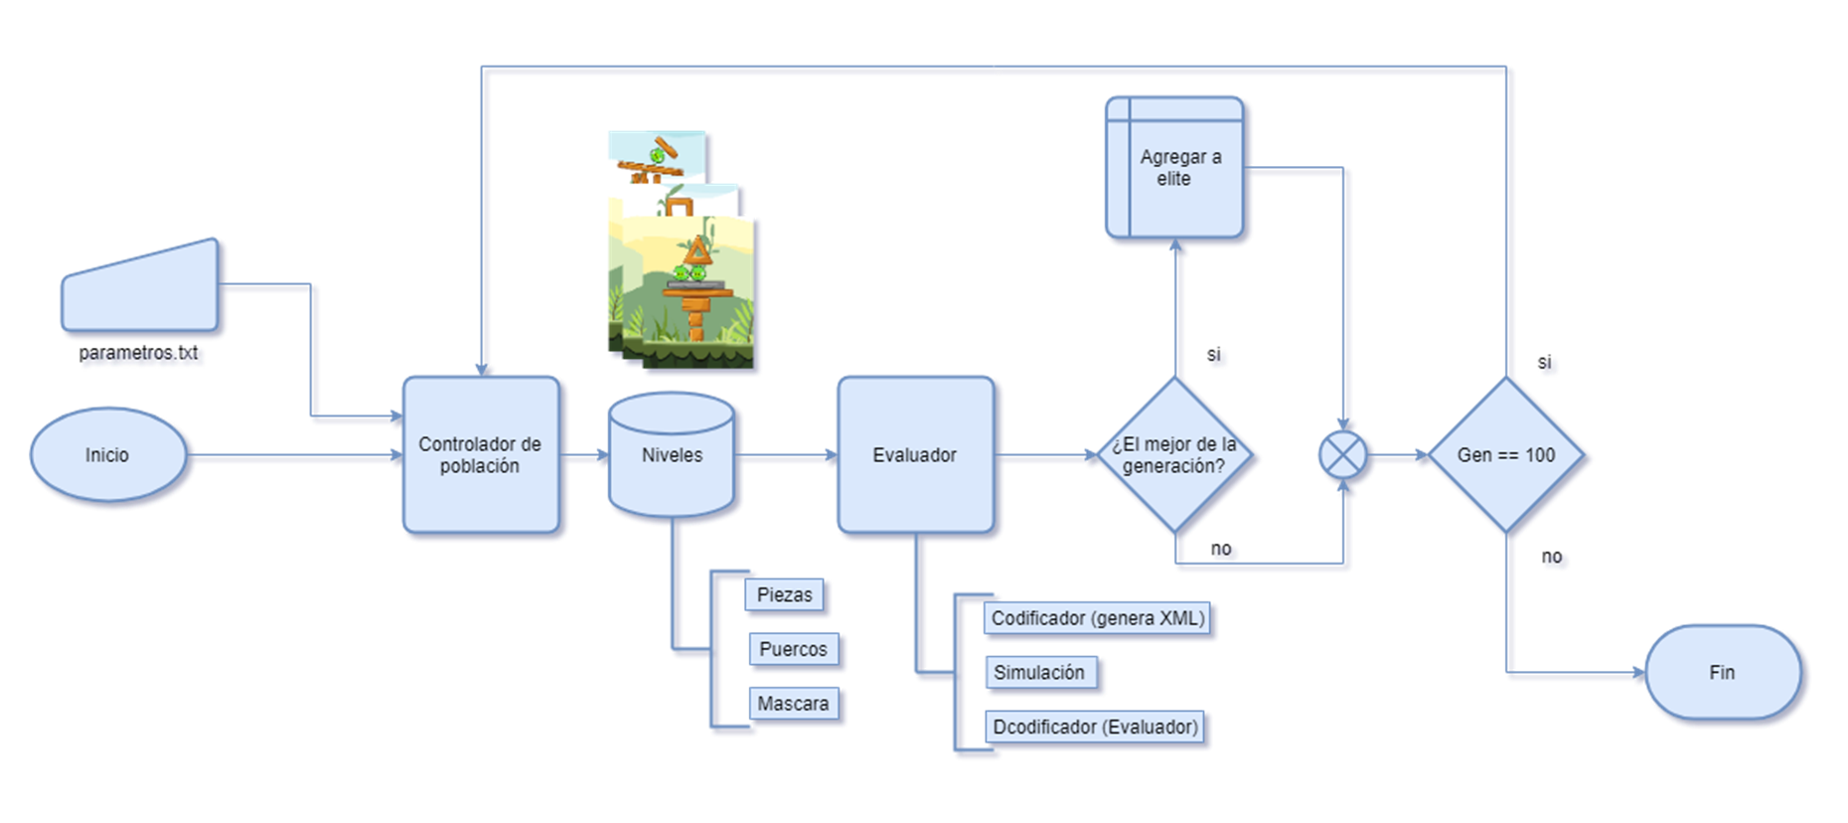
\includegraphics[width=1.0\textwidth]{img/system_model.png}
  \caption{Diagrama de flujo del algoritmo}
  \label{figure:algorithm_model}
\end{figure}

\section{Propuestas anteriores}
\label{section:previous-proposed-methods}

Dentro del aspecto de generar compuestos nuevos para ser utilizados, previamente
se propuso utilizar los resultados de un nivel como compuestos para las
siguientes generaciones, un ejemplo de esto se muestrs en la figura
\ref{figure:prev_composite_proposal_bef_aft} en donde una estructura generada
mediante el algoritmo genetico se simula en el juego y despues de varios
segundos el resultante del mismo podia ser utilizado como un compuesto para la
siguiente generacion, este metodo proveeria una manera de tener compuestos
verificados como viables, sin embargo se opto por utilizar el generador de
compuestos antes de entrar al ciclo del algoritmo genetico.

\begin{figure}
  \centering
  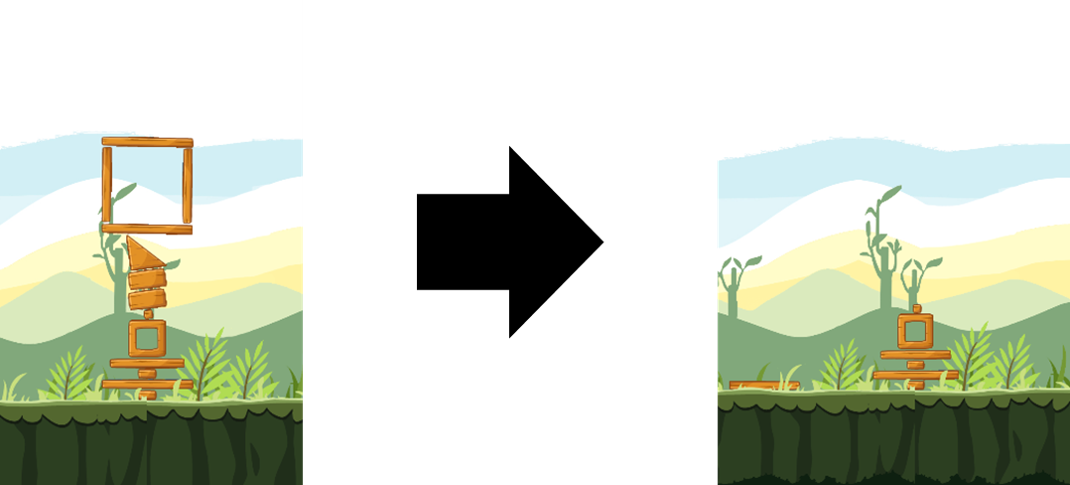
\includegraphics[width=1.0\textwidth]{img/simulation_bef_aft_example.png}
  \caption{Ejemplo de una estructrura antes(izquierda) y despues(derecha) de una simulacion}
  \label{figure:prev_composite_proposal_bef_aft}
\end{figure}

\subsection{Propuesta orientada a metodos}
\label{subsection:objectorientedidea}

Una de las maneras en las que propuso originalmente el desarrollo del proyecto
fue mediante el uso de diccionarios mediante el uso de python, esto permitiria
tener un control de los compuestos generados debido a que mediante el uso de
diccionarios se podia generar un apuntados que permitiria que al momento de
generar los cromosomas de los individuos de la poblacion estos utilizaran
simplemente listas numericas que hicieran referencia al compuesto al cual
pertenecian, esto al final permitiria generar una solo diccionario que
contuviera todos los apuntadores a los compuestos generados.

Esto sin embargo presento un problema para la generacion de nuevos compuestos
debido a que en caso de querer realizar pruebas restringiendo el uso de ciertas
piezas o ciertas combinaciones de material-pieza se tenia que cambiar cada
elemento en el diccionario generado, ademas de esto se requeria de que las
piezas pudieran no solo restringirse sino que se pudieran realizar cambios en
las maneras de como se generaban de manera sencilla, por tal se descarto esta
propuesta con el fin de utilizar la propuesta de generacion de elementos
mediante el uso de clases como se explico en el capitulo
\ref{subsection:classorientedidea}.

Ademas de esto otro de los problemas que se presentaban mediante el uso de
metodos para la generacion de los cromosomas fue que los metodos se asignaban de
manera directa a los individuos lo cual probocaba que simplemente se asignaran
diccionarios que especifican el conjunto de metodos que se deberian de llamar,
sin embargo al no tener los beneficios de un sistema de clases que puede ser
re-instanciado en caso de ser requerido se tiene el problema de que cada que se
realiza una modificacion en los metodos llamados estos cambios se propagan a los
demas individuos provocando errores en los niveles generados.

Uno de los puntos importantes que se lograron rescatar de esta idea fue el uso
de diccionarios para almacenar los valores iniciales de las piezas para permitir
que cada conjunto o compuesto pudiera generarse de manera diferente y que las
piezas en cada uno estarian separadas en relacion a un centro absoluto del
compuesto, ademas de que permite agregar nuevos compuestos de manera rapida lo
cual permite una mejor escalabilidad en la complejidad de los niveles generados.

\subsection{Regla de tercios}
\label{subsection:ruleofthirds}

Uno de los temas que mas interesaba en la generacion de niveles fue la manera en
como se acomodarian las estructuras en al area del juego, debido a que lo que se
busco en el proyecto originalmente fue crear estructuras que tuvieran una gran
altura y lograran mantenerse estables se buscaron maneras de lograr que los
posicionamientos de las piezas o compuestos fuese lo mas \textit{'controlado'}
posible debido a que simplemente colocar piezas al azar generaria demasiado caos
en los niveles generados, por tal motivo una de las primeras propuestas fue el
uso de la \textit{regla de tercios}.

La regla de tercios es una tecnica utilizada en el area de fotografia cuyo
proposito es crear imagenes esteticamente agradables a la vista en donde el
punto focal o punto de interes se encuentra colocado en la alguna de las areas
de la imagen, un ejemplo de esto se puede apreciar en la figura
\ref{figure:ruleofthirdsexample} en donde el objeto principal que se quiere
resaltar se trata de colocar en el area central de la imagen completa.

La regla de tercios es una tecnica utilizada en el area de fotografia cuyo
proposito es crear imagenes balanceadas y esteticamente agradables a la vista,
esto es mediante el uso de lineas imaginarias que dividen la imagen en nueve
areas, la manera en que funciona la regla es que mediante el uso de la
cuadricula generada se colocan los objetos principales de una imagen entre
lineas divisoria de tal manera que en caso de imagenes grandes donde existen dos
o mas elementos importantes un solo objeto no tome el centro absoluto de la
imagen, sino que se mantenga alineado a un punto donde las lineas se cruzan para
que los demas elementos de la imagen tengan un mismo nivel de interes y en el
caso de que solo sea un elementos no utilize toda la parte central de la imagen
sino que exista un nivel de balance en la imagen en donde el cielo o el fondo
tenga una tercera parte del espacio de la fotografia, mientras que el 'area
activa' o el area inmediantamente adyacente al sujeto de la imagen cubra el
resto de la misma.

La manera en como se planeo utilizar esta tecnica es mediante el uso de una
cuadricula de tres por tres de la misma manera que se me muestra en la figura
\ref{figure:ruleofthirdsexample}, pero en el caso de los niveles generados se
espera utilizar la cuadricula para rellenar areas del nivel iniciando desde la
parte inferior para geenerar niveles mas robustos en en sentido de que la
distribucion de las piezas es mas enfocada al centro creando una piramide o
llenando todas las areas dependiendo de la cantidad de piezas utilizadas. 

\begin{figure}
  \centering
  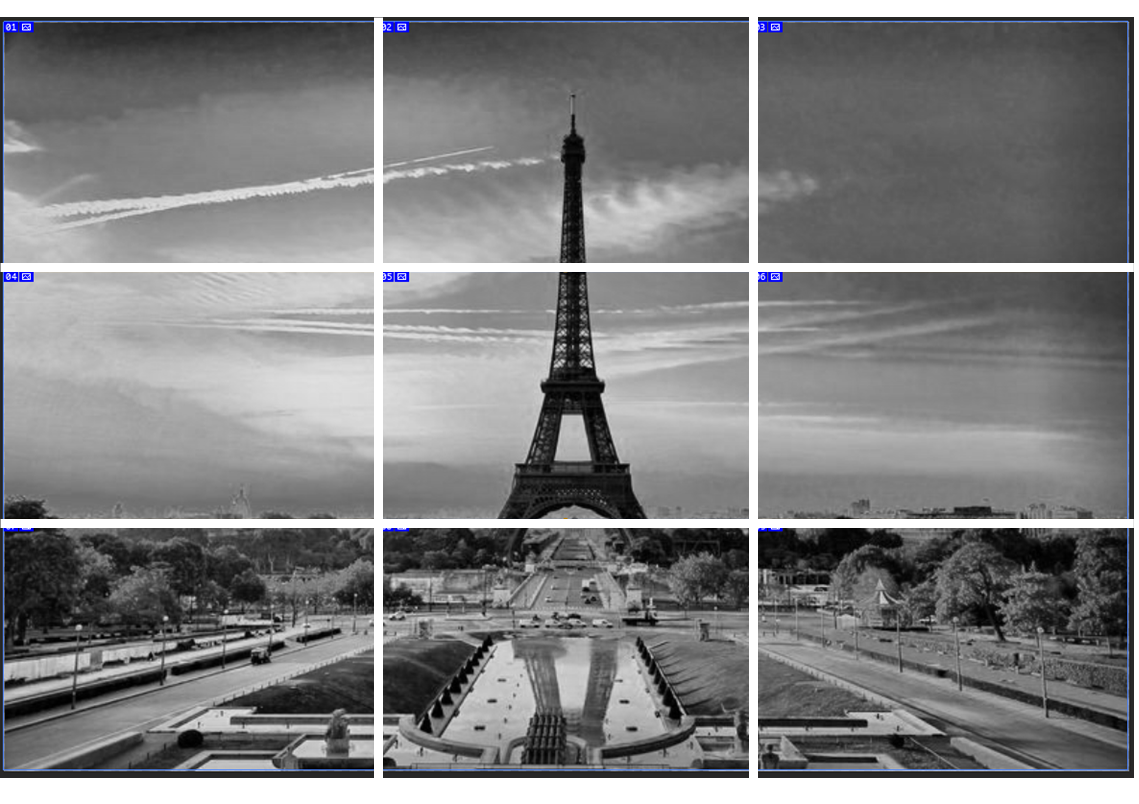
\includegraphics[width=1.0\textwidth]{img/ruleofthirds_example.png}
  \caption{Ejemplo del uso de la regla de tercios en una imagen, el punto de interes se encuentra en la parte central}
  \label{figure:ruleofthirdsexample}
\end{figure}

Debido a que los niveles generados tienen un area de vision o area jugable
variante hasta cierto punto, se definira un area de juego estatica para los
niveles de tal forma que todos siempre se generen con las mismas dimensiones, de
esta manera se evita el tener que estar calculando areas areas para los nueve
cuadrantes utilizando la regla de tercios y se utilizan siempre los mismos
valores para distribuir las piezas en los niveles.

La manera en como se planeo principalmente el uso de la regla de tercios dentro
del proyecto fue mediante el uso de mascaras de generacion, estas mascaras se
generaron mediante la modificacion del la idea detras de la regla de tercios,
esto se utilizo de ugual manera una cuadricula que cubriera el area de juego, la
cuadricula se modifico para cubriera el area con un tamaño de 3 cuadros de
altura y 7 cuadros de largo, de esta manera las piezas tendrian un poco mas de
libertad sobre el donde seria posible colocarlas, el ejemplo basico de la idea
detras del uso de la regla de tercios se muestra en la figura
\ref{figure:ruleofthird_on_pieces} en donde se utiliza una mascara simple para
acomodar los elementos en un individuo de tal manera que el ordenamiento dentro
de la cuadricula permitiria la generacion de estructuras mas complejas, sin
embargo esta idea a pesar de proveeer una buena mecanica en el acomodo de las
piezas conllevaba un error debido que no solo se deberia de buscar los puntos en
los cuales los elementos se podrian apoyar entre ellos, si no que era requerido
tomaer en cuenta las posiciones, alturas, tamaños y angulos de todos los
elementos presentes en el cromosoma una vez colocados en el nivel, los
resultados obtenidos utilizando la regla de tercios se muestran en la figura
\ref{figure:ruleofthird_on_chromosome}, en esta imagen se muestra como una
mascara pre-generada con una forma de castillo mostrada del lado izquiero de la
imagen se combina con el chromosoma entrante de un individuo para generar el
nivel mostrado del lado derecho d ela imagen, este nivel se trata de asemejar a
lo establecido en la mascara, mientras que el uso de mascaras pre-generadas
permite encaminar el sistema de generacion a un conjunto de resultados de igual
manera inhibe que se logre tener una diversidad de niveles debido a que siempre
se mantendran dentro de las formas especificadas por las mascaras, debido a esto
se opto por modificar la idea para permitir que los individiduos tengan una
mascara no pre-generada sino que de manera pseudo-aleatoria se les asigna una
mascara que contendra de igual manera varias columnas en donde el total de
piezas se reparte de manera aleatoria, esto permitira tener mas diversidad en
los niveles generados.

\begin{figure}
  \centering
  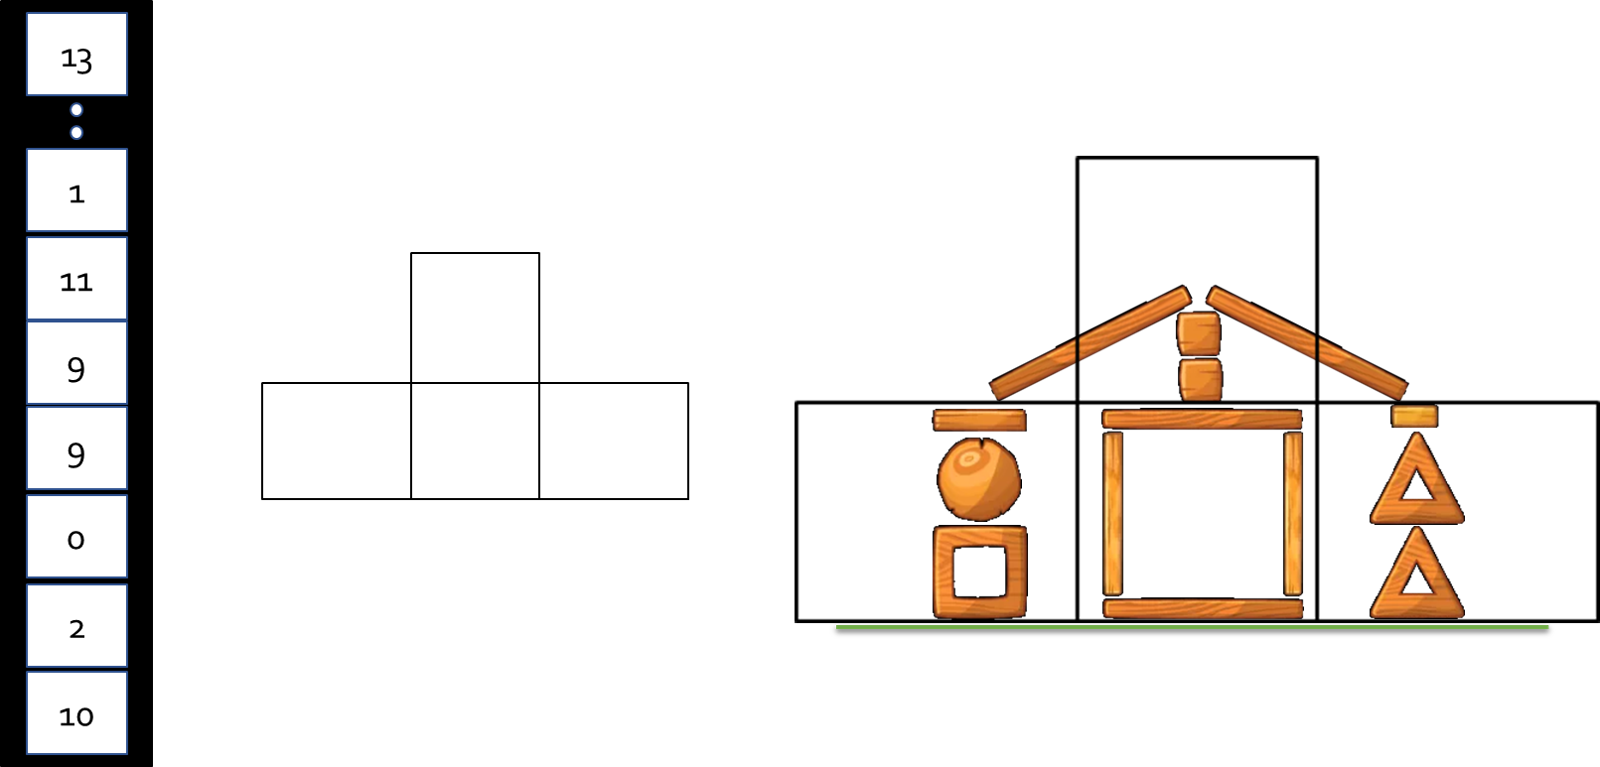
\includegraphics[width=1.0\textwidth]{img/chromosome_thirds.png}
  \caption{Ejemplo del uso de la regla de tercios en un conjunto de piezas, el cromosoma de un individuo(izquierda) se combina con la mascara(centro) para generar una estructura mas compleja(derecha)}
  \label{figure:ruleofthird_on_pieces}
\end{figure}

\begin{figure}
  \centering
  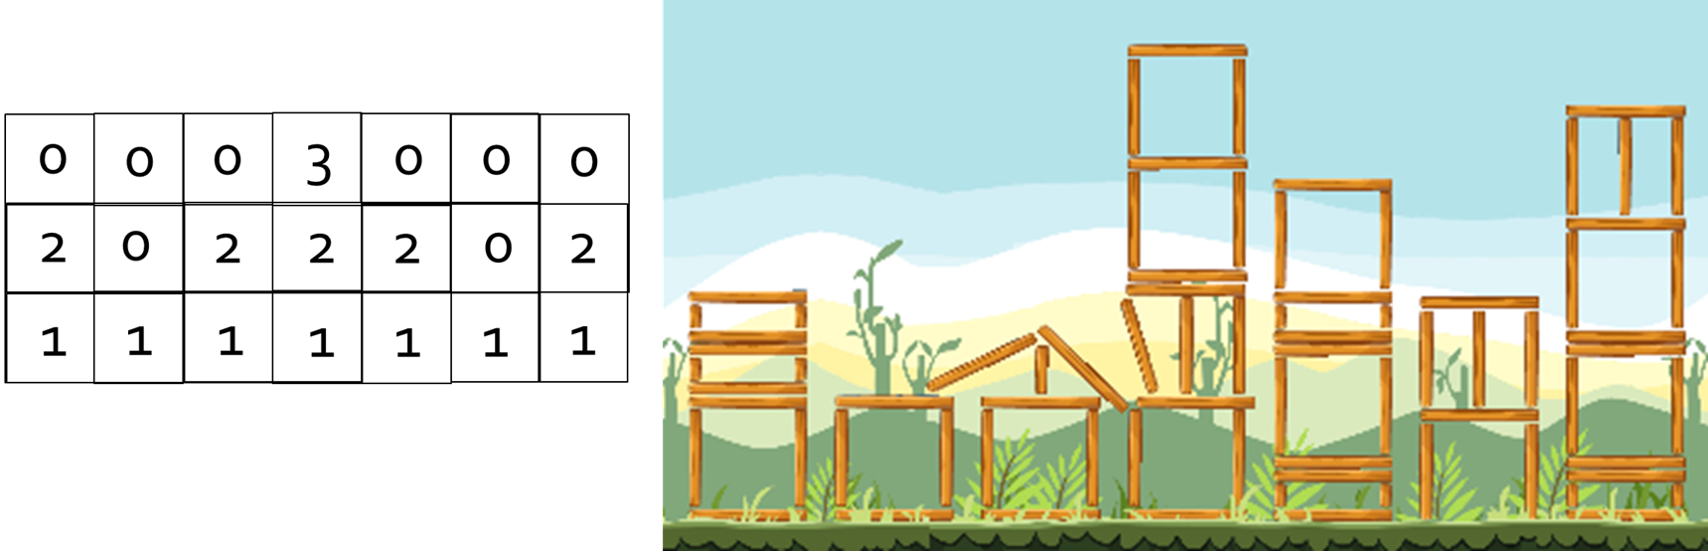
\includegraphics[width=1.0\textwidth]{img/result_example_thirds.png}
  \caption{Resultado obtenido utilizando la regla de tercios, la mascara(izquierda) utilizada y el resultado generado(derecha)}
  \label{figure:ruleofthird_on_chromosome}
\end{figure}

